
%(BEGIN_QUESTION)
% Copyright 2007, Tony R. Kuphaldt, released under the Creative Commons Attribution License (v 1.0)
% This means you may do almost anything with this work of mine, so long as you give me proper credit

A physics professor wants to demonstrate the Ideal Gas Law to his students, so he builds an apparatus consisting of a hollow metal sphere, a small-diameter tube, a bleed valve, and a pressure gauge that looks like this:

$$\includegraphics[width=15.5cm]{i02971x01.eps}$$

First, he immerses the sphere in an ice-water mixture to set the air temperature inside the sphere to 0$^{o}$ C (273.15 K), leaving the bleed valve open to equalize the air pressure inside the sphere with atmospheric.  Next, he closes off the bleed valve to trap air inside the system and plunges the sphere into a beaker full of boiling water (100$^{o}$ C, or 373.15 K).  The pressure gauge indication rises, of course, but it does not fully reach the pressure calculated by the professor using the Ideal Gas Law, even after being left immersed in the boiling water for some time.

\vskip 10pt

Calculate the ``hot'' pressure using the Ideal Gas Law, and express it in units of PSIG.  Also, explain why the pressure registered by the gauge will {\it never} be quite as large as that predicted by the Law.

\vfil 

\underbar{file i02971}
\eject
%(END_QUESTION)





%(BEGIN_ANSWER)

This is a graded question -- no answers or hints given!

%(END_ANSWER)





%(BEGIN_NOTES)

$P_{ideal}$ = 5.38 PSIG

\vskip 10pt

The pressure gauge will never quite reach 5.38 PSIG because not all the air in this closed system has been heated to the boiling temperature of water (373.15 K)!

The experiment may be optimized by using a very large sphere, which works to ``swamp'' the volume contained by the gauge (and tube), but the actual pressure can {\it never precisely} equal the predicted pressure so long as some unheated air remains in the system.

%INDEX% Physics, static fluids: ideal gas law

%(END_NOTES)


